% !TeX root = main.tex

\section{实验结果}

\subsection{实验理论}
本实验的理论内容如图~\ref{fig:mechanism}所示, 硬化水泥石中包含水泥水化产物\ce{Ca(OH)2}, \ce{CSH}, \ce{AFt}, 可能包含未水化的\ce{C2S}与\ce{C3S}. 在加入粉煤灰的水泥石中应该包含不参与反应的粉煤灰.

\begin{figure}[!t]
  \centering
  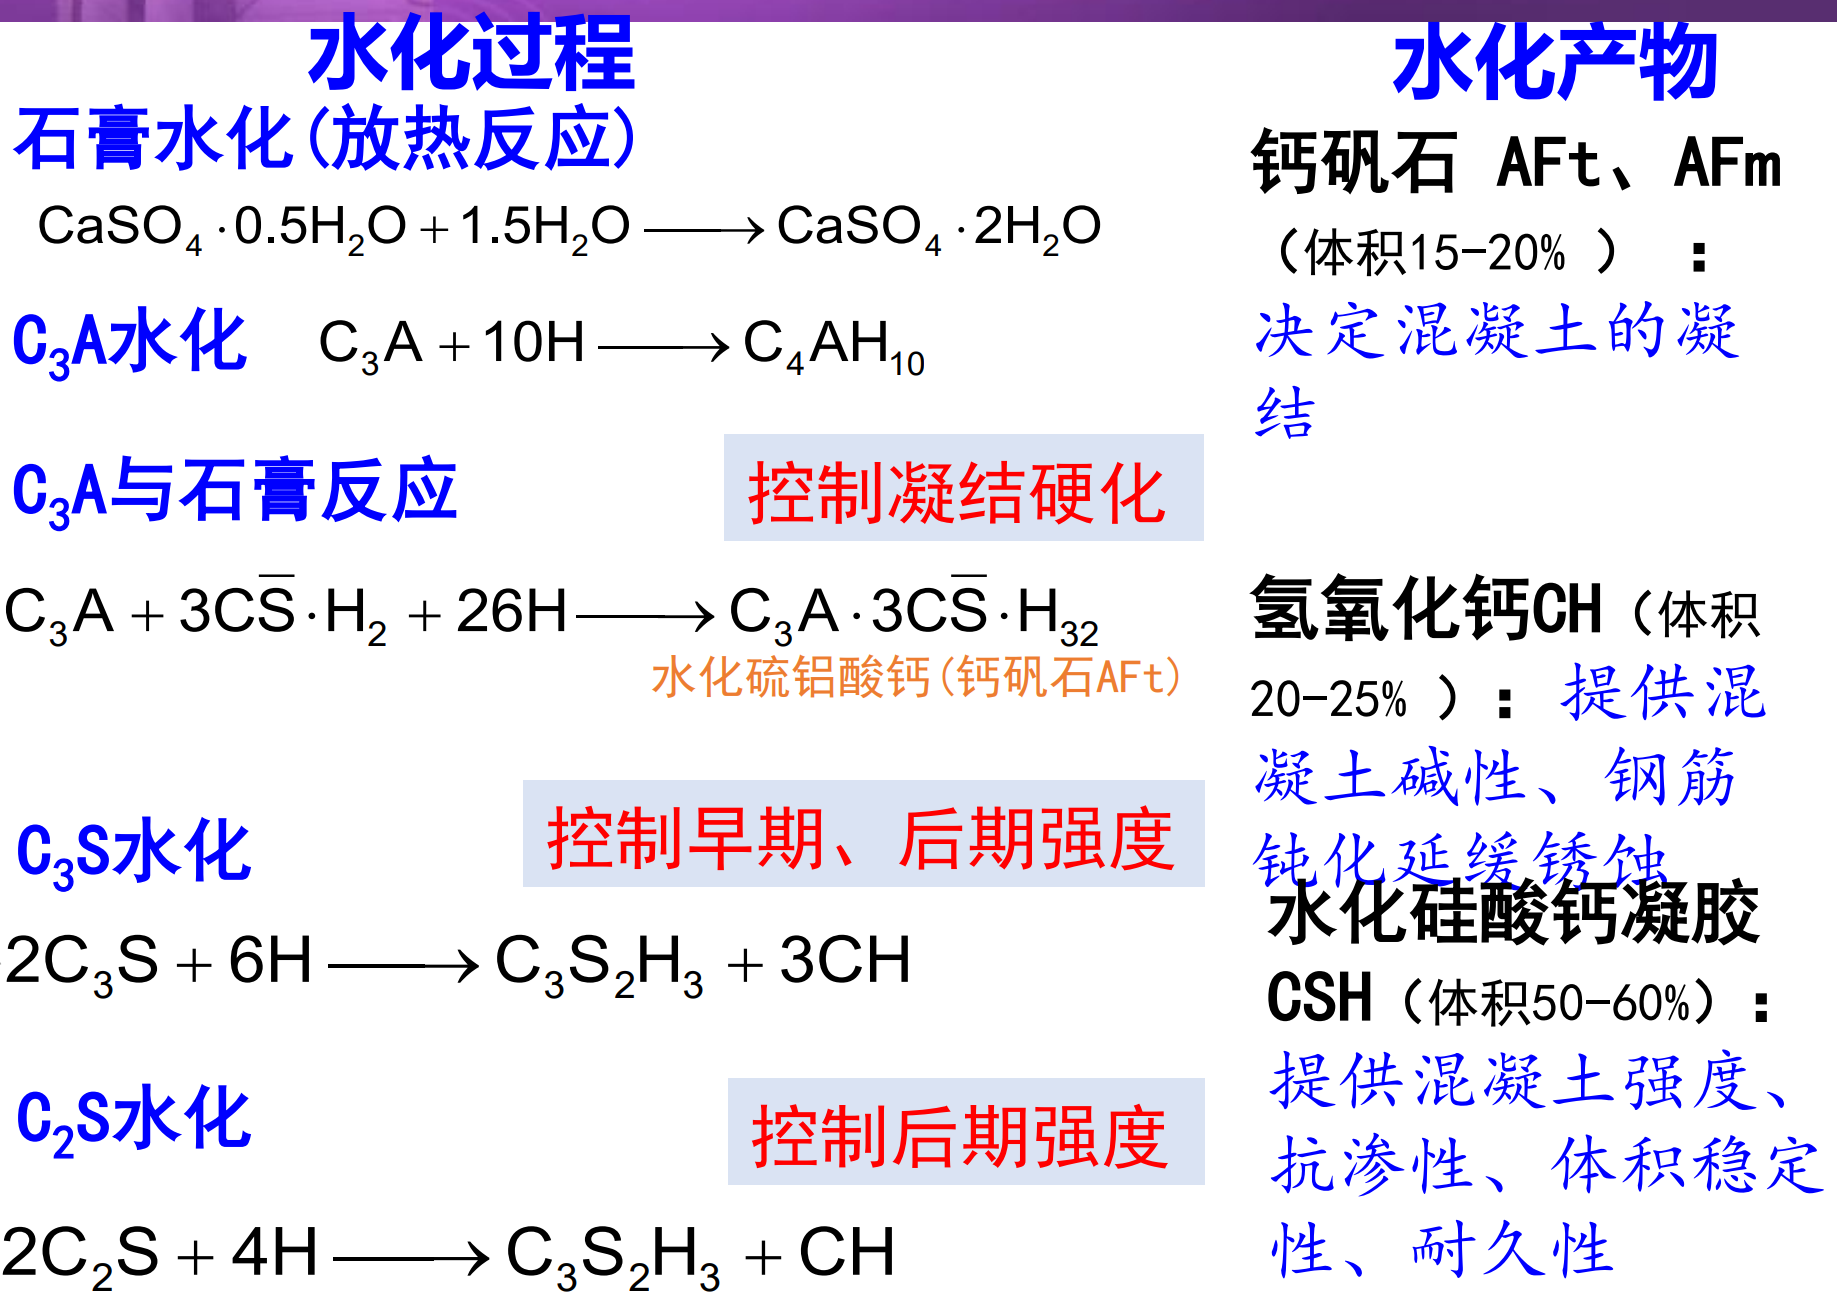
\includegraphics[width = 0.6\linewidth]{figures/exp3/mechanism.png}
  \caption{硬化水泥石中包含的化学反应以及化学物质. 本图来源于孔祥明老师《建筑材料》课程课件. }
  \label{fig:mechanism}
\end{figure}

\subsection{微观结构, 能谱图, 元素组成及成分分析}

\subsubsection{未水化的\ce{C3S}}
\begin{minipage}{\textwidth}
  \begin{minipage}[b]{0.32\textwidth}
    \centering
    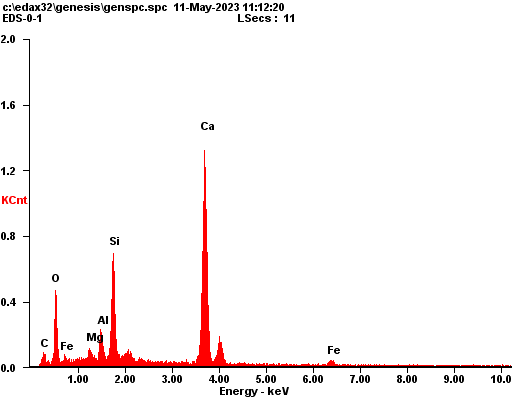
\includegraphics[width = \linewidth]{assets/spectrum/00-01-10000x-ETD-C3S.png}
    \captionof{figure}{粉煤灰掺量0\%, 01区域的能谱图}
  \end{minipage}
  \hfill
  \begin{minipage}[b]{0.32\textwidth}
    \centering
    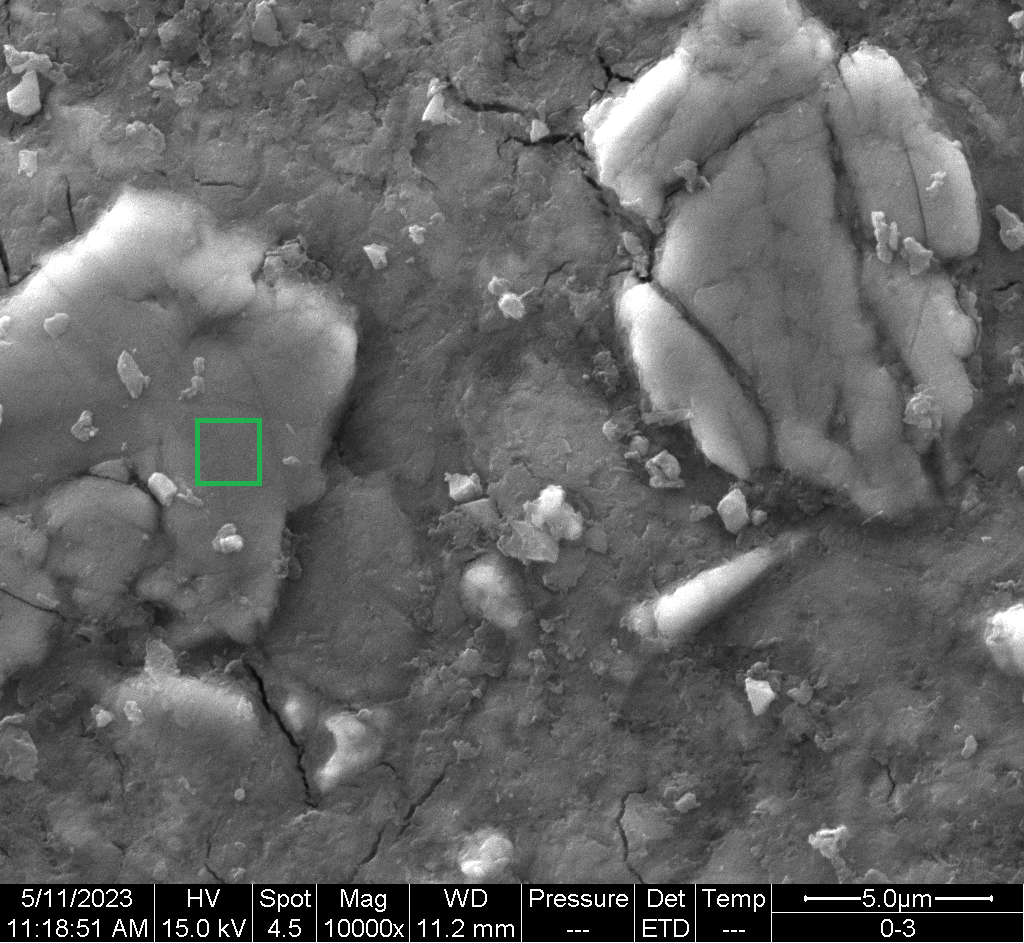
\includegraphics[width = \linewidth]{assets/spectrum selection/00-01-10000x-ETD-C3S.png}
    \captionof{figure}{粉煤灰掺量0\%, 01区域的ETD图像及选择区域}
    \label{fig:00-01-select}
  \end{minipage}
  \hfill
  \begin{minipage}[b]{0.32\textwidth}
    \centering
    \begin{tabular}{|c|c|c|}
      \hline
      Element & Wt \%  & At \%  \\ \hline
      C K     & 03.23 & 06.95 \\ \hline
      O K     & 27.17 & 43.92 \\ \hline
      MgK     & 01.58 & 01.69 \\ \hline
      AlK     & 03.04 & 02.92 \\ \hline
      SiK     & 12.12 & 11.16 \\ \hline
      CaK     & 48.70 & 31.43 \\ \hline
      FeK     & 04.16 & 01.93 \\ \hline
    \end{tabular}
    \captionof{table}{粉煤灰掺量0\%, 01区域的元素组成}
    \label{tab:00-01}
  \end{minipage}
\end{minipage}



\begin{minipage}{\textwidth}
  \begin{minipage}[b]{0.32\textwidth}
    \centering
    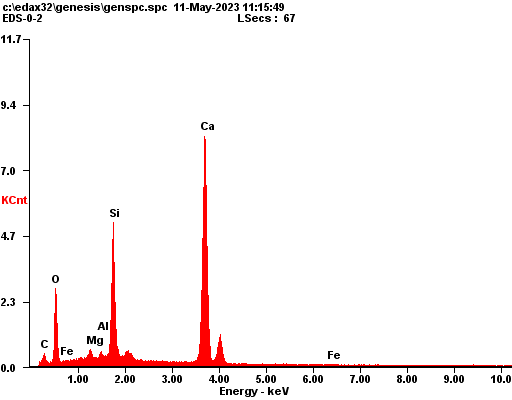
\includegraphics[width = \linewidth]{assets/spectrum/00-02-10000x-ETD-C3S.png}
    \captionof{figure}{粉煤灰掺量0\%, 02区域的能谱图}
  \end{minipage}
  \hfill
  \begin{minipage}[b]{0.32\textwidth}
    \centering
    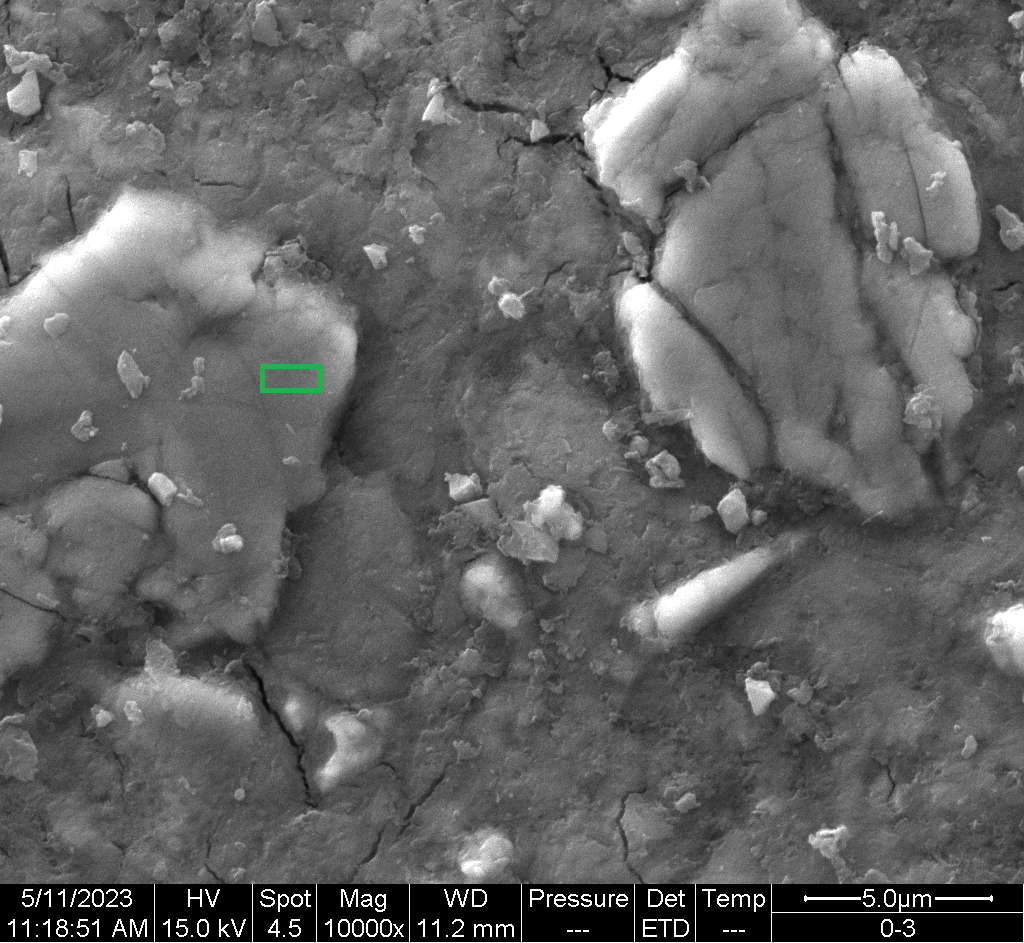
\includegraphics[width = \linewidth]{assets/spectrum selection/00-02-10000x-ETD-C3S.png}
    \captionof{figure}{粉煤灰掺量0\%, 02区域的ETD图像及选择区域}
    \label{fig:00-02-select}
  \end{minipage}
  \hfill
  \begin{minipage}[b]{0.32\textwidth}
    \centering
    \begin{tabular}{|c|c|c|}
    \hline
    Element & Wt \%  & At \%  \\ \hline
    C K     & 02.69 & 05.74 \\ \hline
    O K     & 28.78 & 46.18 \\ \hline
    MgK     & 00.96 & 01.01 \\ \hline
    AlK     & 00.42 & 00.40 \\ \hline
    SiK     & 13.88 & 12.69 \\ \hline
    CaK     & 52.52 & 33.63 \\ \hline
    FeK     & 00.75 & 00.35 \\ \hline
    \end{tabular}
    \captionof{table}{粉煤灰掺量0\%, 02区域的元素组成}
    \label{tab:00-02}
  \end{minipage}
\end{minipage}


在ETD图像中发现了如图~\ref{fig:00-01-select}与图~\ref{fig:00-02-select}的微观结构, 选择以上微观结构区域进行能谱分析, 结果分别如表~\ref{tab:00-01}与表~\ref{tab:00-02}所示. 在表格中, 我们发现\ce{Ca}与\ce{Si}的物质的量之比大约为3:1, 考虑钙, 硅的物质的量之比, 该区域成分应该是\ce{C3S}.

\subsubsection{未水化的\ce{C2S} }

\begin{minipage}{\textwidth}
  \begin{minipage}[b]{0.32\textwidth}
    \centering
    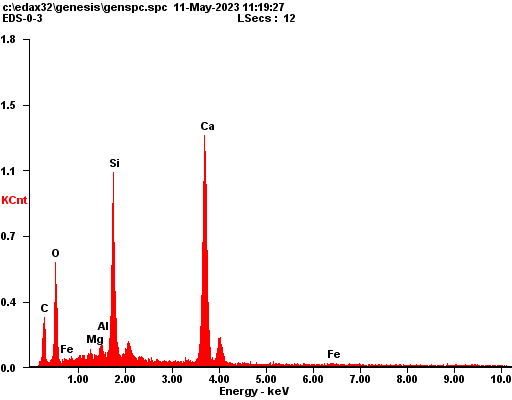
\includegraphics[width = \linewidth]{assets/spectrum/00-03-15000x-ETD-C2S.png}
    \captionof{figure}{粉煤灰掺量0\%, 03区域的能谱图}
  \end{minipage}
  \hfill
  \begin{minipage}[b]{0.32\textwidth}
    \centering
    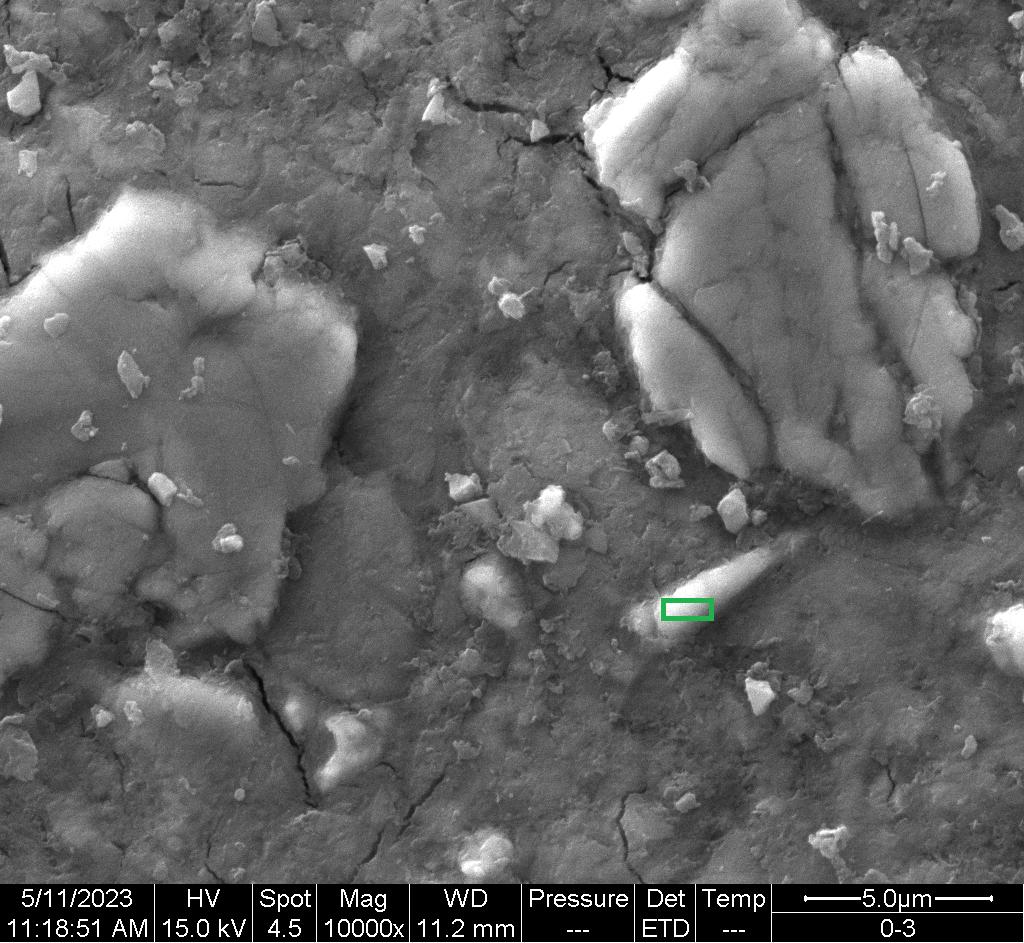
\includegraphics[width = \linewidth]{assets/spectrum selection/00-03-10000x-ETD-C2S.png}
    \captionof{figure}{粉煤灰掺量0\%, 03区域的ETD图像及选择区域}
    \label{fig:00-03-select}
  \end{minipage}
  \hfill
  \begin{minipage}[b]{0.32\textwidth}
    \centering
    \begin{tabular}{|c|c|c|}
      \hline
      Element & Wt \%  & At \%  \\ \hline
      C K     & 10.18 & 19.55 \\ \hline
      O K     & 28.70 & 41.35 \\ \hline
      MgK     & 00.45 & 00.43 \\ \hline
      AlK     & 00.94 & 00.80 \\ \hline
      SiK     & 14.96 & 12.28 \\ \hline
      CaK     & 43.80 & 25.19 \\ \hline
      FeK     & 00.96 & 00.40 \\ \hline
      \end{tabular}
    \captionof{table}{粉煤灰掺量0\%, 03区域的元素组成}
    \label{tab:00-03}
  \end{minipage}
\end{minipage}

在ETD图像中发现了如图~\ref{fig:00-03-select}的微观结构, 选择以上微观结构区域进行能谱分析, 结果分别如表~\ref{tab:00-03}所示. 在表格中, 我们发现\ce{Ca}与\ce{Si}的物质的量之比大约为2:1, 考虑钙, 硅的物质的量之比, 该区域成分应该是\ce{C2S}.


\subsubsection{水化产物\ce{CH} 或 \ce{Ca(OH)2} }

\begin{minipage}{\textwidth}
  \begin{minipage}[b]{0.32\textwidth}
    \centering
    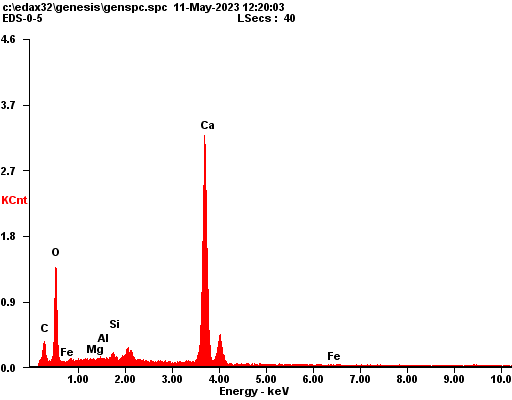
\includegraphics[width = \linewidth]{assets/spectrum/00-05-10000x-ETD-CH.png}
    \captionof{figure}{粉煤灰掺量0\%, 05区域的能谱图}
  \end{minipage}
  \hfill
  \begin{minipage}[b]{0.32\textwidth}
    \centering
    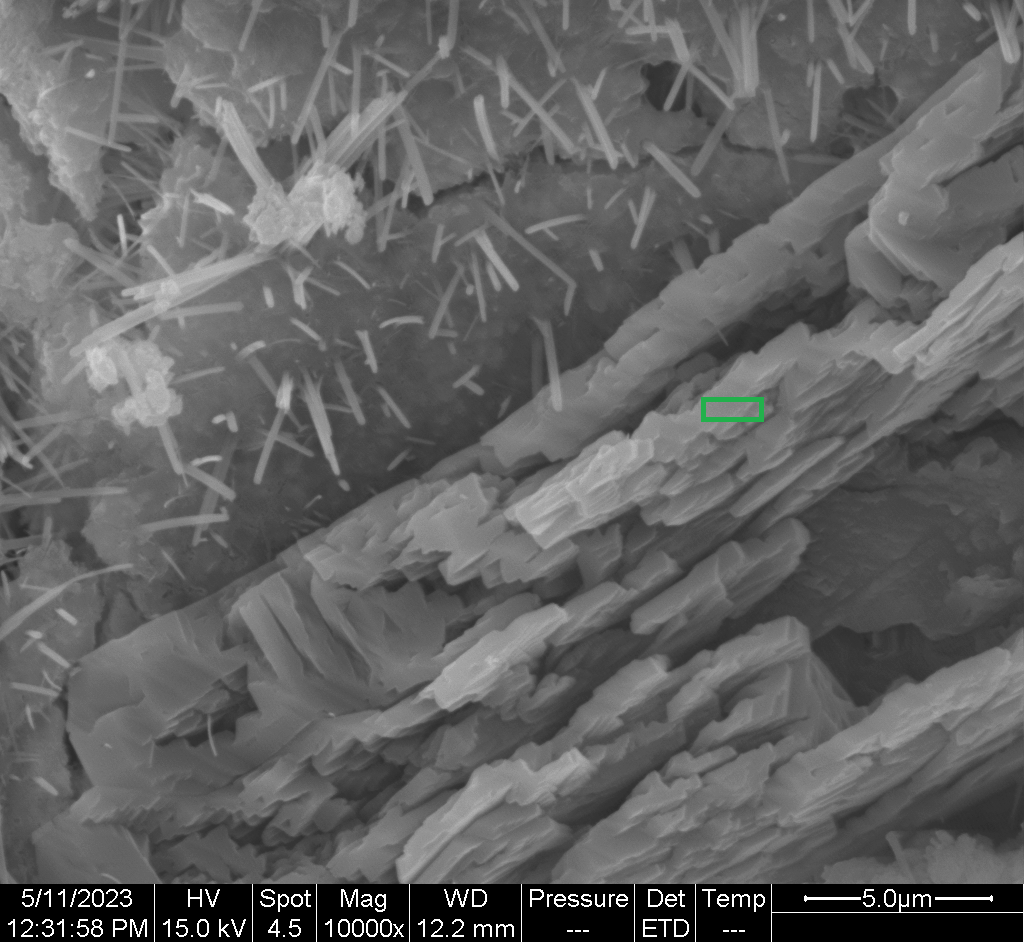
\includegraphics[width = \linewidth]{assets/spectrum selection/00-05-10000x-ETD-CH.png}
    \captionof{figure}{粉煤灰掺量0\%, 05区域的ETD图像及选择区域}
    \label{fig:00-05-select}
  \end{minipage}
  \hfill
  \begin{minipage}[b]{0.32\textwidth}
    \centering
    \begin{tabular}{|c|c|c|}
      \hline

      Element & Wt \%  & At \%  \\ \hline
      C K     & 02.24 & 05.37 \\ \hline
      O K     & 22.10 & 39.79 \\ \hline
      MgK     & 00.30 & 00.36 \\ \hline
      AlK     & 00.41 & 00.44 \\ \hline
      SiK     & 00.90 & 00.93 \\ \hline
      CaK     & 73.53 & 52.85 \\ \hline
      FeK     & 00.52 & 00.27 \\ \hline
      \end{tabular}
    \captionof{table}{粉煤灰掺量0\%, 05区域的元素组成}
    \label{tab:00-05}
  \end{minipage}
\end{minipage}


\begin{minipage}{\textwidth}
  \begin{minipage}[b]{0.32\textwidth}
    \centering
    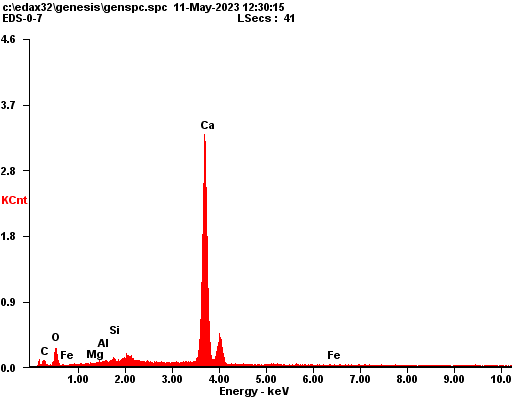
\includegraphics[width = \linewidth]{assets/spectrum/00-07-10000x-ETD-CH.png}
    \captionof{figure}{粉煤灰掺量0\%, 07区域的能谱图}
  \end{minipage}
  \hfill
  \begin{minipage}[b]{0.32\textwidth}
    \centering
    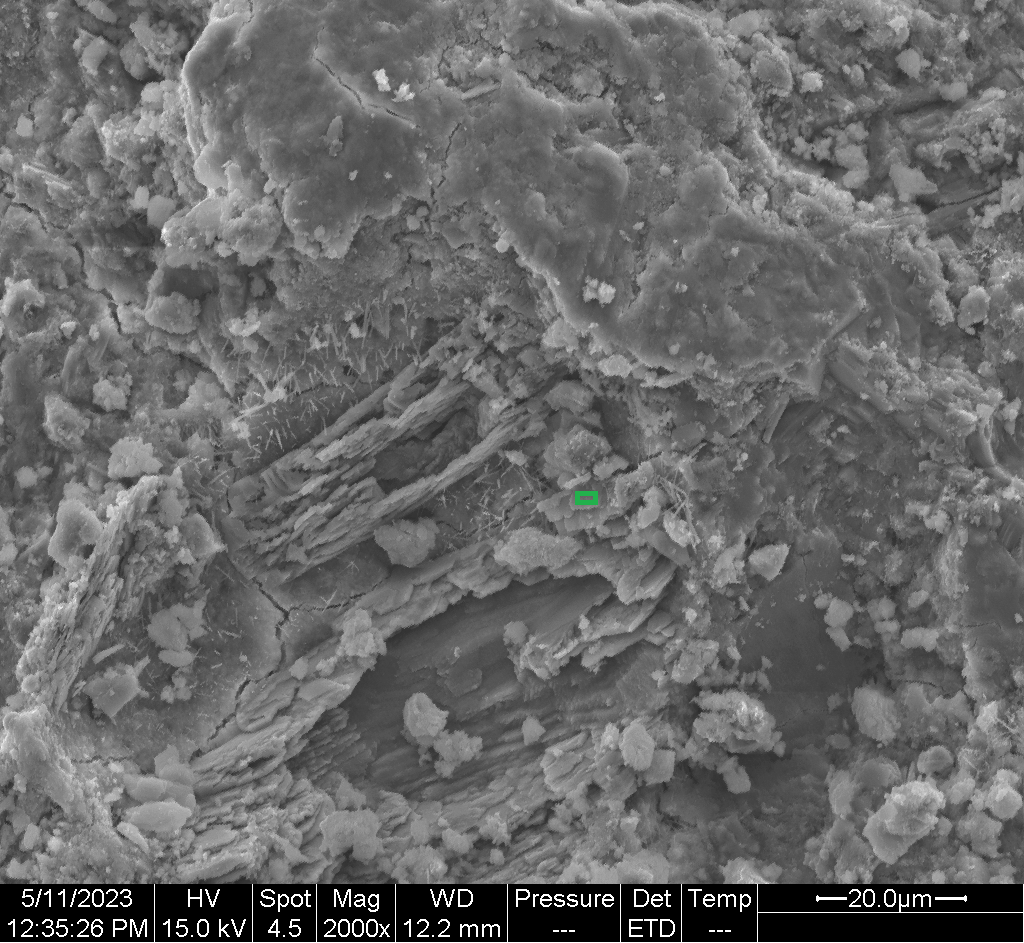
\includegraphics[width = \linewidth]{assets/spectrum selection/00-07-02000x-ETD-CH.png}
    \captionof{figure}{粉煤灰掺量0\%, 07区域的ETD图像及选择区域}
    \label{fig:00-07-select}
  \end{minipage}
  \hfill
  \begin{minipage}[b]{0.32\textwidth}
    \centering
    \begin{tabular}{|c|c|c|}
      \hline
      Element & Wt \%  & At \%  \\ \hline
      C K     & 01.37 & 03.63 \\ \hline
      O K     & 14.85 & 29.56 \\ \hline
      MgK     & 00.11 & 00.15 \\ \hline
      AlK     & 00.34 & 00.40 \\ \hline
      SiK     & 00.86 & 00.98 \\ \hline
      CaK     & 81.36 & 64.65 \\ \hline
      FeK     & 01.09 & 00.62 \\ \hline
      \end{tabular}
    \captionof{table}{粉煤灰掺量0\%, 07区域的元素组成}
    \label{tab:00-07}
  \end{minipage}
\end{minipage}

在ETD图像中发现了如图~\ref{fig:00-05-select}和图~\ref{fig:00-07-select}的片层状微观结构, 选择以上微观结构区域进行能谱分析, 结果分别如表~\ref{tab:00-05}和表~\ref{tab:00-07}所示. 在表格中, 我们发现在表格中主要的元素组成为\ce{Ca}与\ce{O}, 而\ce{Si}等其他元素很少, 推测该区域成分是\ce{CH}, 即\ce{Ca(OH)2}.

\subsubsection{水化产物\ce{CSH}}

\begin{minipage}{\textwidth}
  \begin{minipage}[b]{0.32\textwidth}
    \centering
    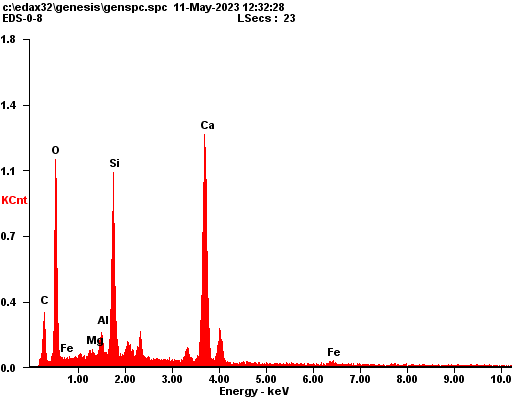
\includegraphics[width = \linewidth]{assets/spectrum/00-08-10000x-ETD-CSH.png}
    \captionof{figure}{粉煤灰掺量0\%, 08区域的能谱图}
  \end{minipage}
  \hfill
  \begin{minipage}[b]{0.32\textwidth}
    \centering
    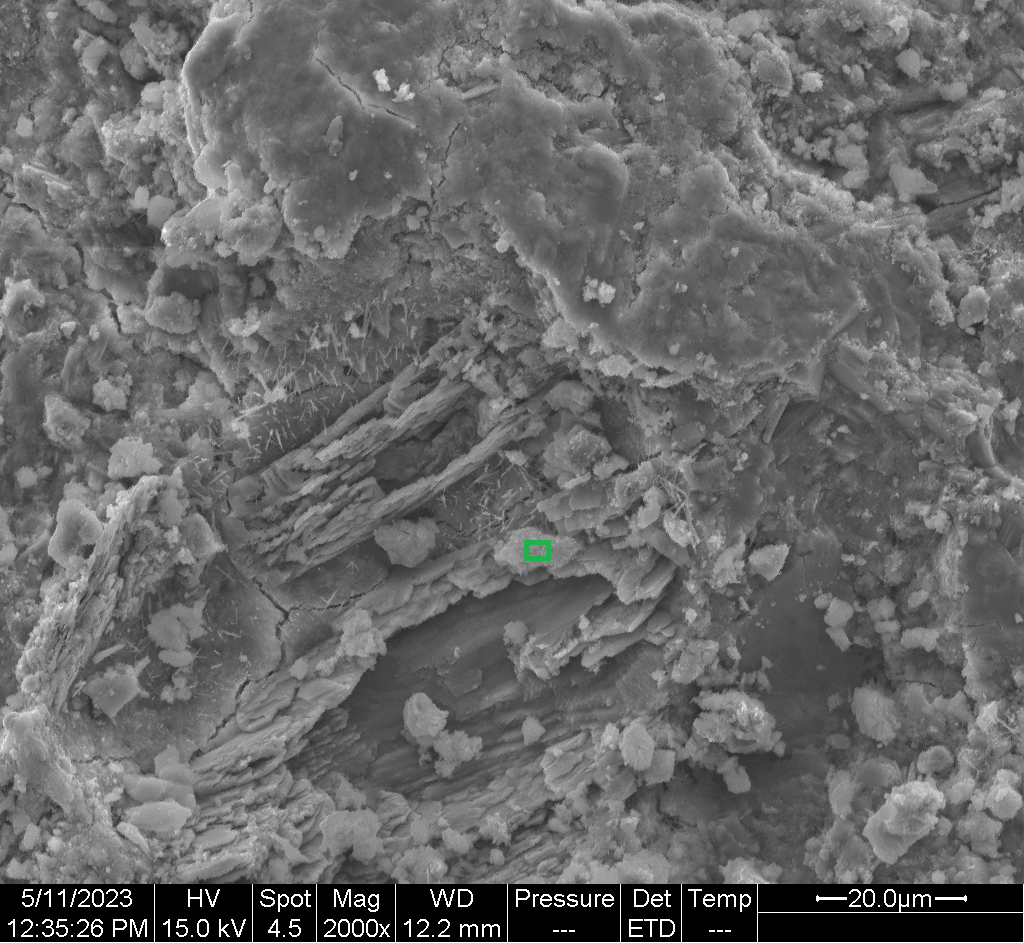
\includegraphics[width = \linewidth]{assets/spectrum selection/00-08-02000x-ETD-CSH.png}
    \captionof{figure}{粉煤灰掺量0\%, 08区域的ETD图像及选择区域}
    \label{fig:00-08-select}
  \end{minipage}
  \hfill
  \begin{minipage}[b]{0.32\textwidth}
    \centering
    \begin{tabular}{|c|c|c|}
      \hline
      Element & Wt \%  & At \%  \\ \hline
      C K     & 08.04 & 14.52 \\ \hline
      O K     & 40.04 & 54.29 \\ \hline
      MgK     & 00.48 & 00.43 \\ \hline
      AlK     & 01.49 & 01.20 \\ \hline
      SiK     & 12.39 & 09.57 \\ \hline
      CaK     & 35.43 & 19.17 \\ \hline
      FeK     & 02.13 & 00.83 \\ \hline
      \end{tabular}
    \captionof{table}{粉煤灰掺量0\%, 08区域的元素组成}
    \label{tab:00-08}
  \end{minipage}
\end{minipage}


\begin{minipage}{\textwidth}
  \begin{minipage}[b]{0.32\textwidth}
    \centering
    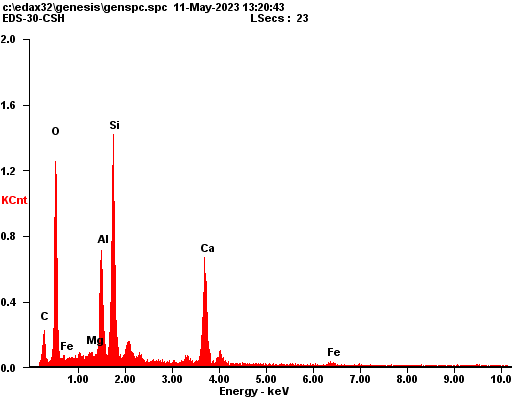
\includegraphics[width = \linewidth]{assets/spectrum/30-01-30000x-ETD-CSH.png}
    \captionof{figure}{粉煤灰掺量30\%, 01区域的能谱图}
  \end{minipage}
  \hfill
  \begin{minipage}[b]{0.32\textwidth}
    \centering
    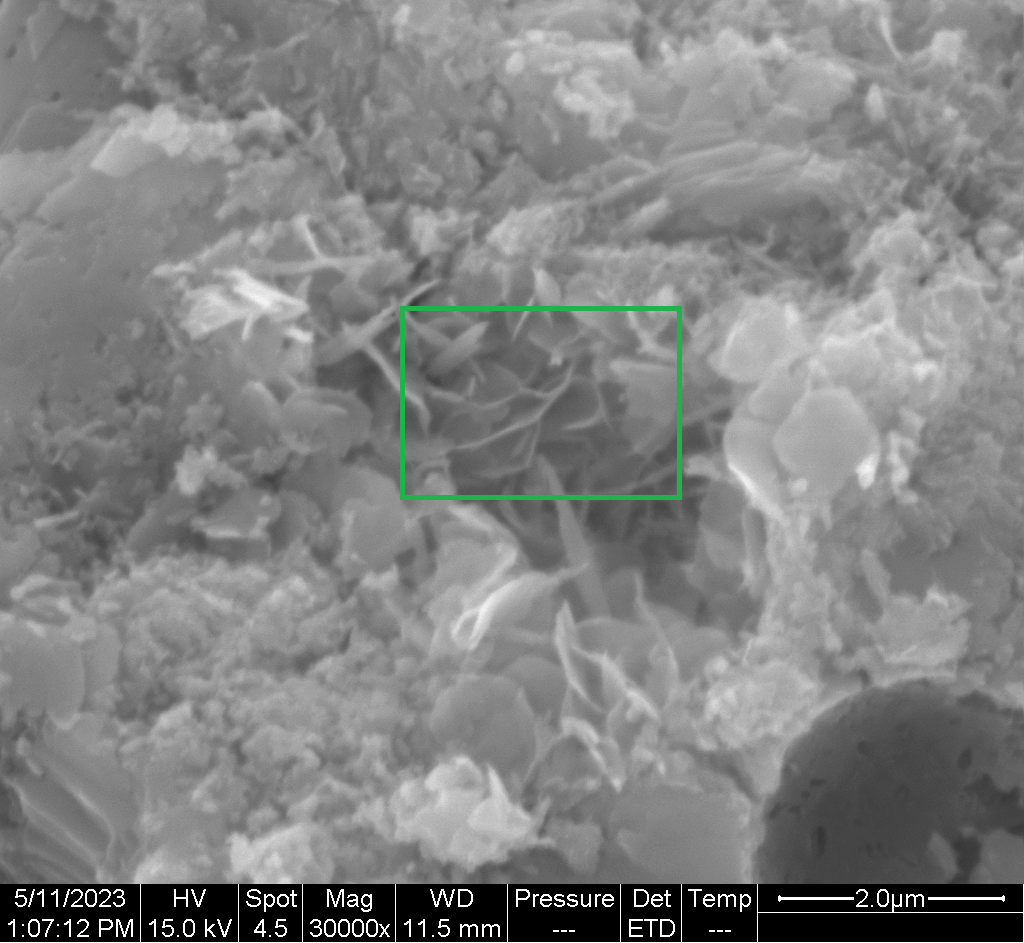
\includegraphics[width = \linewidth]{assets/spectrum selection/30-01-30000x-CSH.png}
    \captionof{figure}{粉煤灰掺量30\%, 01区域的ETD图像及选择区域}
    \label{fig:30-01-select}
  \end{minipage}
  \hfill
  \begin{minipage}[b]{0.32\textwidth}
    \centering
    \begin{tabular}{|c|c|c|}
    \hline
    Element & Wt \%  & At \%  \\ \hline
    C K     & 09.18 & 15.71 \\ \hline
    O K     & 40.78 & 52.38 \\ \hline
    MgK     & 00.43 & 00.36 \\ \hline
    AlK     & 08.57 & 06.53 \\ \hline
    SiK     & 19.82 & 14.50 \\ \hline
    CaK     & 18.75 & 09.61 \\ \hline
    FeK     & 02.47 & 00.91 \\ \hline
    \end{tabular}
    \captionof{table}{粉煤灰掺量30\%, 01区域的元素组成}
    \label{tab:30-01}
  \end{minipage}
\end{minipage}

在ETD图像中发现了如图~\ref{fig:00-08-select}和图~\ref{fig:30-01-select}的网络状微观结构, 选择以上微观结构区域进行能谱分析, 结果如表~\ref{tab:00-08}和表~\ref{tab:30-01}所示. 在图中, 我们发现该微观结构并没有规则的结构, 也不存在规律性, 因此排除其为晶体的可能性; 同时, 由于其体积尺寸超出\SI{10}{\micro\meter} , 因而推断其属于\ce{CSH}. 同时, 在表格中, 我们发现在表格中主要的元素组成为\ce{Ca}, \ce{Si} 与 \ce{O}, 且\ce{O} 元素成分极大, 推测该区域成分是\ce{CSH} 凝胶.
\wei{最好对CSH做一些定量的分析, 通过其At\% 来分析. }

\begin{figure}
  \centering
  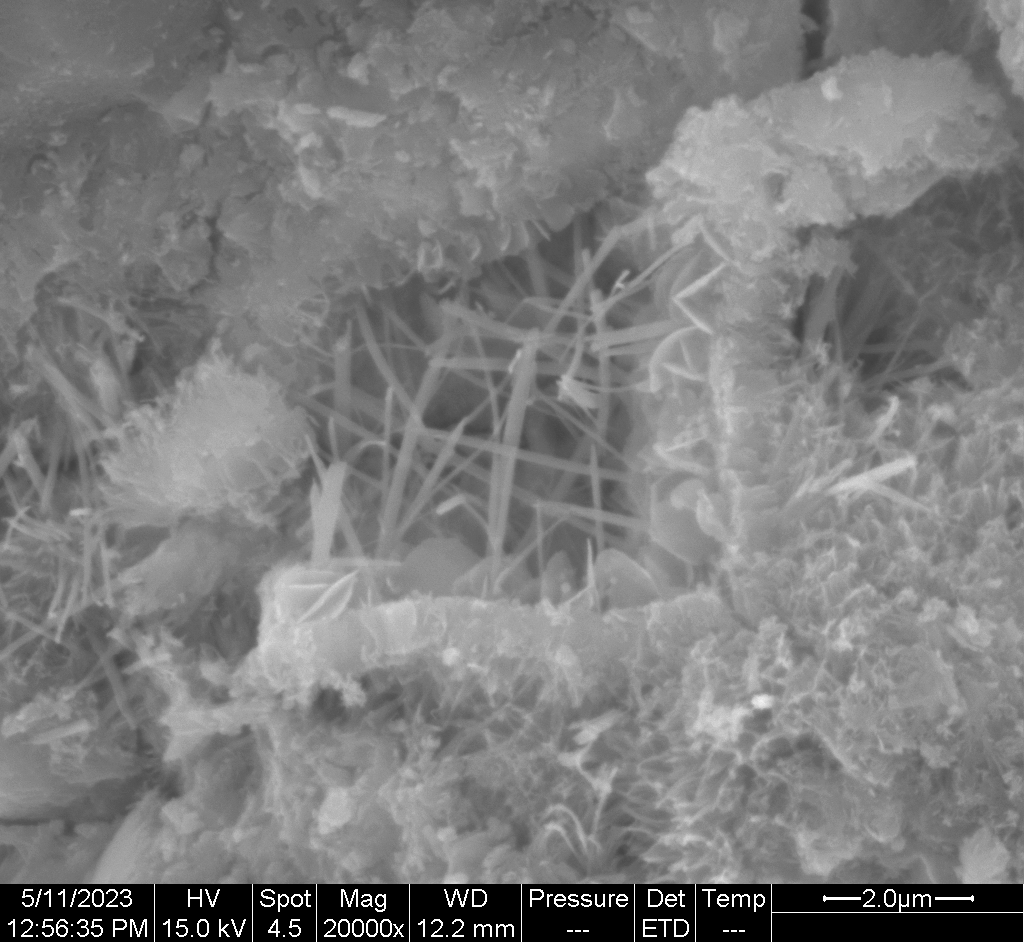
\includegraphics[width=0.5\textwidth]{assets/15-unpolished-20000x-ETD.png}
  \caption{粉煤灰掺量15\%, 未抛光的硬化水泥石, 在20000x倍率下的ETD图像. }
  \label{fig:ETD-CSH}
\end{figure}

更细致的网络结构如图~\ref{fig:ETD-CSH}所示.

\subsubsection{水化产物\ce{AFt}}

在ETD图像中发现了如图~\ref{fig:00-05-select}左上方所示的针棒状微观结构, 发现其微观结构规则, 认为其属于晶体; 考虑到其针棒状结构, 推测其属于钙矾石\ce{AFt}. 然而, 遗憾的是, 由于其分布区域过小, 无法选择区域对其做能谱分析, 进行验证.

\subsubsection{粉煤灰}

\begin{minipage}{\textwidth}
  \begin{minipage}[b]{0.32\textwidth}
    \centering
    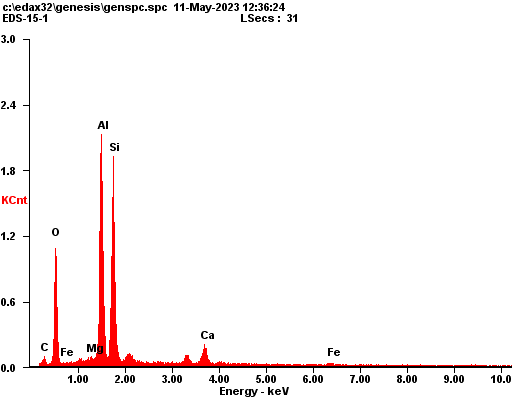
\includegraphics[width = \linewidth]{assets/spectrum/15-01-4000x-ETD-FA.png}
    \captionof{figure}{粉煤灰掺量15\%, 01区域的能谱图}
  \end{minipage}
  \hfill
  \begin{minipage}[b]{0.32\textwidth}
    \centering
    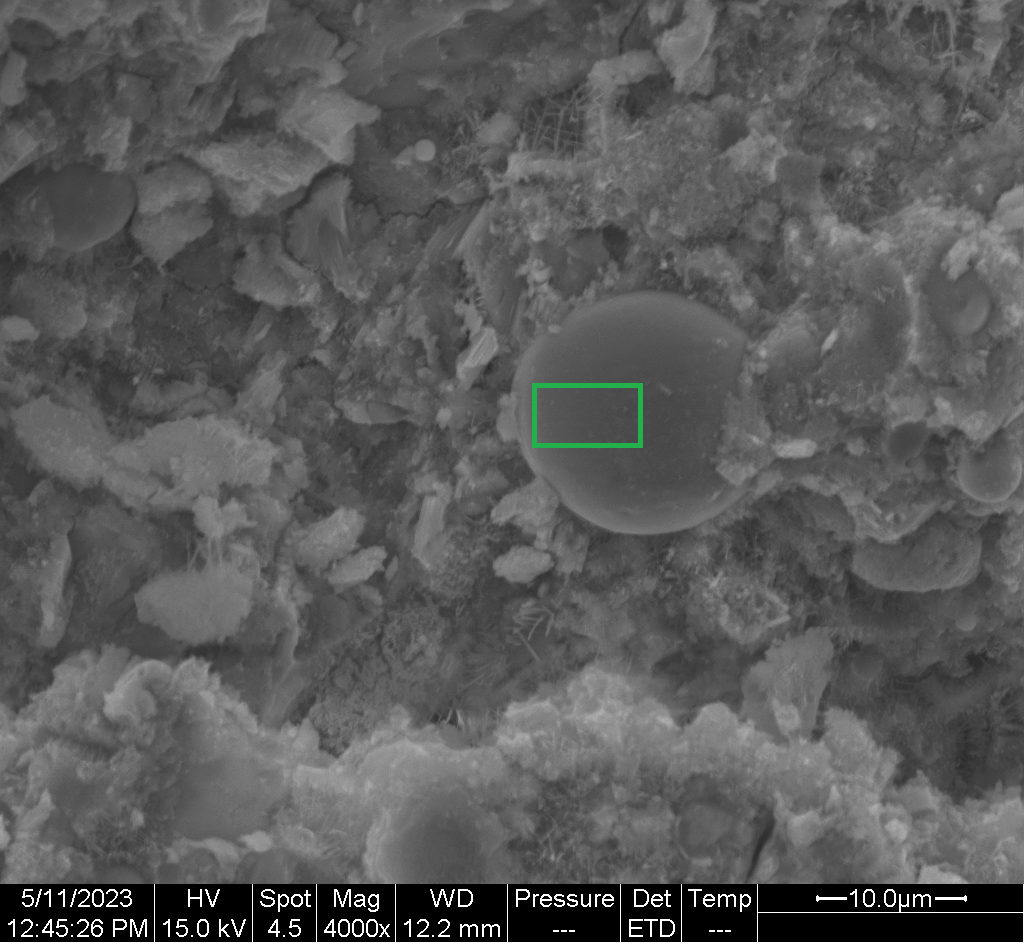
\includegraphics[width = \linewidth]{assets/spectrum selection/15-01-04000x-ETD-FA.png}
    \captionof{figure}{粉煤灰掺量15\%, 01区域的ETD图像及选择区域}
    \label{fig:15-01-select}
  \end{minipage}
  \hfill
  \begin{minipage}[b]{0.32\textwidth}
    \centering
    \begin{tabular}{|c|c|c|}
      \hline
      Element & Wt \%  & At \%  \\ \hline
      C K     & 05.53 & 10.11 \\ \hline
      O K     & 29.58 & 40.58 \\ \hline
      MgK     & 00.46 & 00.41 \\ \hline
      AlK     & 26.03 & 21.17 \\ \hline
      SiK     & 30.33 & 23.70 \\ \hline
      CaK     & 05.58 & 03.05 \\ \hline
      FeK     & 02.48 & 00.98 \\ \hline
      \end{tabular}
    \captionof{table}{粉煤灰掺量15\%, 01区域的元素组成}
    \label{tab:15-01}
  \end{minipage}
\end{minipage}

在ETD图像中发现了如图~\ref{fig:15-01-select}的球形的微观结构, 选择以上微观结构区域进行能谱分析, 结果如表~\ref{tab:15-01}所示. 我们发现在表格中主要的元素组成为\ce{Si}, \ce{Al} 与 \ce{O}, 且含有一定量的\ce{C} ; 而粉煤灰主要成分为粉煤灰主要成分是硅铝酸钙, 且钙的含量一般较低, 由于粉煤灰是火电厂的产品, 可能含有\ce{C}, 而且因而认为该区域成分是粉煤灰.

\wei{粉煤灰实际上会参与火山灰反应. 前 \SI{7}{\day} 的时候, 可以认为粉煤灰暂时不会参与反应, 即, 其火山灰反应速率较慢, 很难看出其变化. 在水泥养护的后期, 或者更长的时间内, 理论上来说, 火山灰反应会不断进行, 增强后期的强度. 在微观层面上, 前 \SI{7}{\day} 的粉煤灰呈球形, 边界清晰; 从理论上来讲, 随着火山灰反应的进行, 在后期, 粉煤灰的球形边界会慢慢模糊, 逐渐与周边融为一体. }

\begin{figure}[!t]
  \centering
  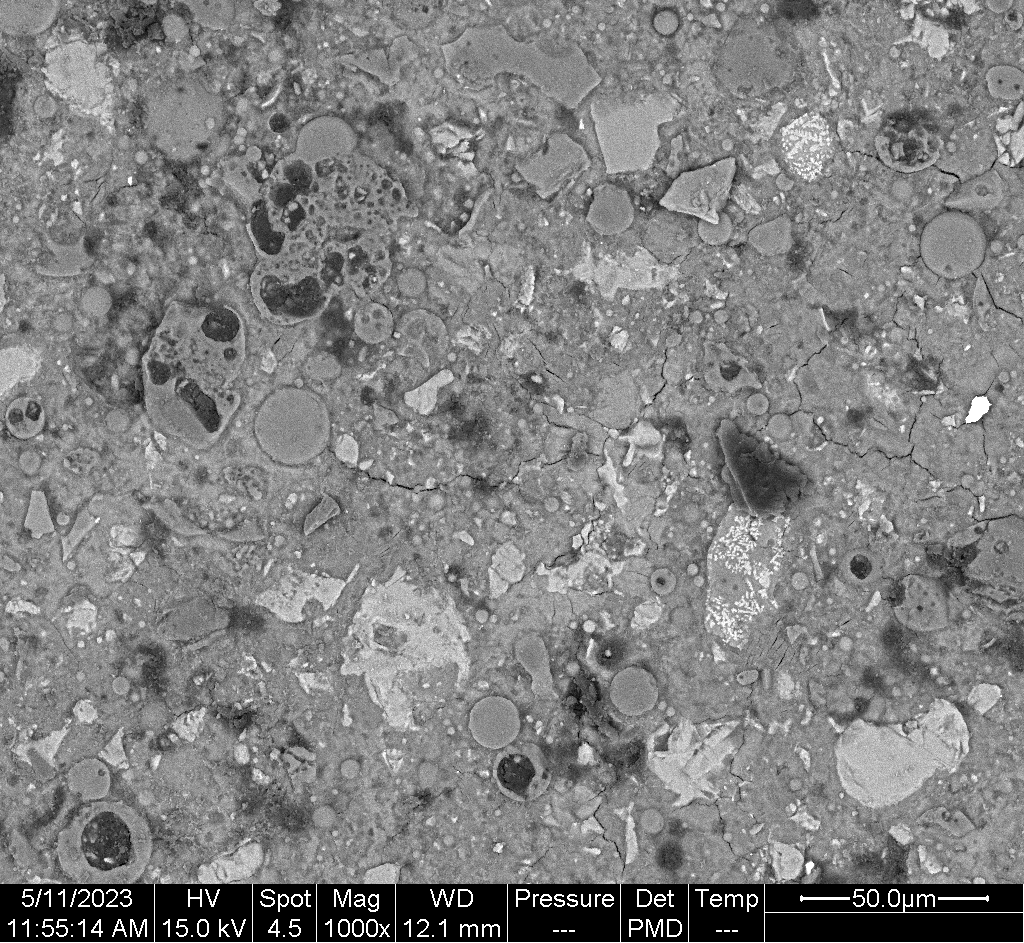
\includegraphics[width = 0.5\textwidth]{assets/30-polished-01000x-PMD.png}
  \caption{粉煤灰掺量30\%, 抛光后的硬化水泥块, 在1000x放大倍率下的背散射图. }
  \label{fig:BSE-FA}
\end{figure}

同样地, 我们在 PMD 图像中发现了如图~\ref{fig:BSE-FA}中的圆形微观结构, 认为其为粉煤灰. 其中具有黑色的物质经推测为碳粉.
